\newpage
\section{Nutation}
Bei diesem Teil des Versuches wurde ein Kreisel bei bekannter Rotationsfrequenz in eine Nutationsbewegung gebracht.
Anschließend wurde die Nutationsdauer für 10 Umdrehungen bestimmt.
Diese Messung wurde jeweils zwei mal für 11 Frequenzen (\(10\,\text{Hz}-20\,\text{Hz}\)) durchgeführt.
Es ergibt sich folgende Wertetabelle:
\begin{table}[h]
    \centering\begin{tabular}{c|c|c|c}
        Rotationsfrequenz $\omega_3$ in Hz & Messung 1 $T_{\text{n}_{10}}$ in s & Messung 2 $T_{\text{n}_{10}}$ in s & Messung 3 $T_{\text{n}_{10}}$ in s\\
        \hline
        10&57,88&57,54&57,62\\
        11&52,16&54,29&53,10\\
        12&50,78&50,38&-\\
        13&47,31&47,40&-\\
        14&46,03&43,22&44,63\\
        15&40,59&40,60&-\\
        16&36,66&36,63&-\\
        17&34,07&34,63&-\\
        18&30,75&30,88&-\\
        19&29,18&29,41&-\\
        20&27,31&27,16&-
    \end{tabular}
    \caption{Wertetabelle: Nutation}
\end{table}
Bei manchen Rotationsfrequenzen wurde ein drittes mal gemessen, da die vorangeganenen Messungen etwas auseinander lagen.\\
Nun wird jeweils der Mittelwert aus den Nutationsdauern ($T_{\text{n}_{10}}$) bestimmt.\\
Somit folgt diese Wertetabelle:
\begin{center}
    \begin{tabular}{c|c}
        $f_3$ in Hz&$\overline{T_{\text{n}_{10}}}$ in s \\
        \hline
        10&57,680\\
        11&53,183\\
        12&50,580\\
        13&47,355\\
        14&44,627\\
        15&40,595\\
        16&36,645\\
        17&34,350\\
        18&30,815\\
        19&29,295\\
        20&27,235
    \end{tabular} 
\end{center}
Der Fehler von $\overline{T_{\text{n}_{10}}}$ ist der Ablesefehler der Stoppuhr.
Da jeweils 10 Umdrehungen gemessen wurden, beträgt der Fehler für eine Umdrehung nur $\frac{1}{10}$ des Ablesefehlers.
Dieser wurde etwas größer Abgeschätz, da man noch die Reaktionszeit der Messperson und den ungenauen Nulldurchgang nicht genau festmachen kann.
Der Fehler für die Rotationsfrequenz ist gleich dem Ablesefehler des Stroposkops:
\begin{align*}
    s_{\overline{T_{\text{n}_{10}}}}&=0,5\,\text{s}\\
    s_{\omega_{3}}&=2\cdot\pi\cdot0,5\,\text{Hz}\\
\end{align*} 
Nun wird jeweils $\omega_\text{n}$ für eine Rotationsfrequenz bestimmt:
\begin{align*}
    \omega_\text{n}&=\frac{2\pi}{\overline{T_{\text{n}_{10}}}}\cdot 10\\
    s_{\omega_\text{n}}&=\frac{20\pi}{\left(\overline{T_{\text{n}_{10}}}\right)^2}\cdot s_{\overline{T_{\text{n}_{10}}}}
\end{align*}
Es ergibt sich folgende Tabelle:
\begin{center}
    \begin{tabular}{c|c|c}
        $\overline{T_{\text{n}_{10}}}$ in s & $\omega_\text{n}$ in Hz & $s_{\omega_\text{n}}$\\
        \hline
        57,680&1,0893178&0,0094428\\
        53,183&1,1814274&0,0111072\\
        50,580&1,2422272&0,0122798\\
        47,355&1,3268262&0,0140094\\
        44,627&1,4079336&0,0157745\\
        40,595&1,5477732&0,0190636\\
        36,645&1,7146092&0,0233949\\
        34,350&1,8291660&0,0266254\\
        30,815&2,0390022&0,0330846\\
        29,295&2,1447979&0,0366069\\
        27,235&2,3070260&0,0423541
    \end{tabular}
\end{center}
Nun soll das Verhältnis aus $\omega_\text{n}$ und $\omega_3$ gegen $\omega_3$ in einem Diagramm gegen $\omega_3$ aufgetragen werden.
Desweiteren ist folgendes gegeben:
\begin{equation*}
    \frac{\omega_\text{n}}{\omega_3}=\frac{J_3-J_1}{J_1}
\end{equation*}
Da \(J_1>J_3\) ist, muss das Verhältnis negativ sein.
Für die Berechung des Fehler des Verhältnisses folgt:
\begin{align*}
    V&=\frac{\omega_\text{n}}{\omega_3}\\
    s_{V}&=\sqrt{\left(\frac{\partial V}{\partial \omega_3}\cdot s_{\omega_3}\right)^2+\left(\frac{\partial V}{\partial \omega_\text{n}}\cdot s_{\omega_\text{n}}\right)^2}\\
    &=\sqrt{\left(\frac{\omega_\text{n}}{\left(\omega_3\right)^2}\cdot s_{\omega_3}\right)^2+\left(\frac{s_{\omega_\text{n}}}{\omega_3}\right)^2}
\end{align*}\newpage
Es folgt die Wertetabelle mit den berechneten Werten:
\begin{table}[ht]
    \centering\begin{tabular}{c|c|c|c}
      $\frac{\omega_\text{n}}{\omega_3}$ & $s_{\frac{\omega_\text{n}}{\omega_3}}$ & $\omega_3$ in Hz & $s_{\omega_3}$ in Hz\\
      \hline
      -0,017337032&0,0008797827&62,83185307&3,141592654\\
        -0,017093637&0,0007934291&69,11503838&3,141592654\\
        -0,016475550&0,0007055366&75,39822369&3,141592654\\
        -0,016243919&0,0006478805&81,68140899&3,141592654\\
        -0,016005685&0,0005991002&87,96459430&3,141592654\\
        -0,016422384&0,0005835875&94,24777961&3,141592654\\
        -0,017055533&0,0005815744&100,5309649&3,141592654\\
        -0,017124754&0,0005619765&106,8141502&3,141592654\\
        -0,018028738&0,0005799774&113,0973355&3,141592654\\
        -0,017966062&0,0005635244&119,3805208&3,141592654\\
        -0,018358730&0,0005694294&125,6637061&3,141592654
    \end{tabular}
    \caption{Wertetabelle: Nutationsfrequenz}
\end{table}\\
Somit ergibt sich folgender Plot:
\begin{figure}[h]
    \centering\scalebox{0.85}{% GNUPLOT: LaTeX picture with Postscript
\begingroup
  % Encoding inside the plot.  In the header of your document, this encoding
  % should to defined, e.g., by using
  % \usepackage[cp1252,<other encodings>]{inputenc}
  \inputencoding{cp1252}%
  \makeatletter
  \providecommand\color[2][]{%
    \GenericError{(gnuplot) \space\space\space\@spaces}{%
      Package color not loaded in conjunction with
      terminal option `colourtext'%
    }{See the gnuplot documentation for explanation.%
    }{Either use 'blacktext' in gnuplot or load the package
      color.sty in LaTeX.}%
    \renewcommand\color[2][]{}%
  }%
  \providecommand\includegraphics[2][]{%
    \GenericError{(gnuplot) \space\space\space\@spaces}{%
      Package graphicx or graphics not loaded%
    }{See the gnuplot documentation for explanation.%
    }{The gnuplot epslatex terminal needs graphicx.sty or graphics.sty.}%
    \renewcommand\includegraphics[2][]{}%
  }%
  \providecommand\rotatebox[2]{#2}%
  \@ifundefined{ifGPcolor}{%
    \newif\ifGPcolor
    \GPcolorfalse
  }{}%
  \@ifundefined{ifGPblacktext}{%
    \newif\ifGPblacktext
    \GPblacktexttrue
  }{}%
  % define a \g@addto@macro without @ in the name:
  \let\gplgaddtomacro\g@addto@macro
  % define empty templates for all commands taking text:
  \gdef\gplbacktext{}%
  \gdef\gplfronttext{}%
  \makeatother
  \ifGPblacktext
    % no textcolor at all
    \def\colorrgb#1{}%
    \def\colorgray#1{}%
  \else
    % gray or color?
    \ifGPcolor
      \def\colorrgb#1{\color[rgb]{#1}}%
      \def\colorgray#1{\color[gray]{#1}}%
      \expandafter\def\csname LTw\endcsname{\color{white}}%
      \expandafter\def\csname LTb\endcsname{\color{black}}%
      \expandafter\def\csname LTa\endcsname{\color{black}}%
      \expandafter\def\csname LT0\endcsname{\color[rgb]{1,0,0}}%
      \expandafter\def\csname LT1\endcsname{\color[rgb]{0,1,0}}%
      \expandafter\def\csname LT2\endcsname{\color[rgb]{0,0,1}}%
      \expandafter\def\csname LT3\endcsname{\color[rgb]{1,0,1}}%
      \expandafter\def\csname LT4\endcsname{\color[rgb]{0,1,1}}%
      \expandafter\def\csname LT5\endcsname{\color[rgb]{1,1,0}}%
      \expandafter\def\csname LT6\endcsname{\color[rgb]{0,0,0}}%
      \expandafter\def\csname LT7\endcsname{\color[rgb]{1,0.3,0}}%
      \expandafter\def\csname LT8\endcsname{\color[rgb]{0.5,0.5,0.5}}%
    \else
      % gray
      \def\colorrgb#1{\color{black}}%
      \def\colorgray#1{\color[gray]{#1}}%
      \expandafter\def\csname LTw\endcsname{\color{white}}%
      \expandafter\def\csname LTb\endcsname{\color{black}}%
      \expandafter\def\csname LTa\endcsname{\color{black}}%
      \expandafter\def\csname LT0\endcsname{\color{black}}%
      \expandafter\def\csname LT1\endcsname{\color{black}}%
      \expandafter\def\csname LT2\endcsname{\color{black}}%
      \expandafter\def\csname LT3\endcsname{\color{black}}%
      \expandafter\def\csname LT4\endcsname{\color{black}}%
      \expandafter\def\csname LT5\endcsname{\color{black}}%
      \expandafter\def\csname LT6\endcsname{\color{black}}%
      \expandafter\def\csname LT7\endcsname{\color{black}}%
      \expandafter\def\csname LT8\endcsname{\color{black}}%
    \fi
  \fi
    \setlength{\unitlength}{0.0500bp}%
    \ifx\gptboxheight\undefined%
      \newlength{\gptboxheight}%
      \newlength{\gptboxwidth}%
      \newsavebox{\gptboxtext}%
    \fi%
    \setlength{\fboxrule}{0.5pt}%
    \setlength{\fboxsep}{1pt}%
\begin{picture}(7200.00,5040.00)%
    \gplgaddtomacro\gplbacktext{%
      \csname LTb\endcsname%%
      \put(1342,704){\makebox(0,0)[r]{\strut{}$-0.019$}}%
      \csname LTb\endcsname%%
      \put(1342,1218){\makebox(0,0)[r]{\strut{}$-0.0185$}}%
      \csname LTb\endcsname%%
      \put(1342,1733){\makebox(0,0)[r]{\strut{}$-0.018$}}%
      \csname LTb\endcsname%%
      \put(1342,2247){\makebox(0,0)[r]{\strut{}$-0.0175$}}%
      \csname LTb\endcsname%%
      \put(1342,2761){\makebox(0,0)[r]{\strut{}$-0.017$}}%
      \csname LTb\endcsname%%
      \put(1342,3276){\makebox(0,0)[r]{\strut{}$-0.0165$}}%
      \csname LTb\endcsname%%
      \put(1342,3790){\makebox(0,0)[r]{\strut{}$-0.016$}}%
      \csname LTb\endcsname%%
      \put(1342,4305){\makebox(0,0)[r]{\strut{}$-0.0155$}}%
      \csname LTb\endcsname%%
      \put(1342,4819){\makebox(0,0)[r]{\strut{}$-0.015$}}%
      \csname LTb\endcsname%%
      \put(1548,484){\makebox(0,0){\strut{}$60$}}%
      \csname LTb\endcsname%%
      \put(2283,484){\makebox(0,0){\strut{}$70$}}%
      \csname LTb\endcsname%%
      \put(3018,484){\makebox(0,0){\strut{}$80$}}%
      \csname LTb\endcsname%%
      \put(3753,484){\makebox(0,0){\strut{}$90$}}%
      \csname LTb\endcsname%%
      \put(4488,484){\makebox(0,0){\strut{}$100$}}%
      \csname LTb\endcsname%%
      \put(5223,484){\makebox(0,0){\strut{}$110$}}%
      \csname LTb\endcsname%%
      \put(5958,484){\makebox(0,0){\strut{}$120$}}%
      \csname LTb\endcsname%%
      \put(6693,484){\makebox(0,0){\strut{}$130$}}%
    }%
    \gplgaddtomacro\gplfronttext{%
      \csname LTb\endcsname%%
      \put(209,2761){\rotatebox{-270}{\makebox(0,0){\strut{}$\frac{\omega_n}{\omega_3}$}}}%
      \csname LTb\endcsname%%
      \put(6748,2761){\rotatebox{-270}{\makebox(0,0){\strut{}}}}%
      \csname LTb\endcsname%%
      \put(4083,154){\makebox(0,0){\strut{}$\omega_3\,(\text{Hz})$}}%
      \csname LTb\endcsname%%
      \put(4083,4819){\makebox(0,0){\strut{}}}%
      \csname LTb\endcsname%%
      %\put(-2147483648,20470){\makebox(0,0){\strut{}}}%
      %\csname LTb\endcsname%%
      \put(132,-110){\makebox(0,0)[l]{\strut{}}}%
      \csname LTb\endcsname%%
      \put(5706,4646){\makebox(0,0)[r]{\strut{}Messung}}%
      \csname LTb\endcsname%%
      \put(5706,4426){\makebox(0,0)[r]{\strut{}fit}}%
      \csname LTb\endcsname%%
      \put(4083,45380){\makebox(0,0){\strut{}}}%
    }%
    \gplbacktext
    \put(0,0){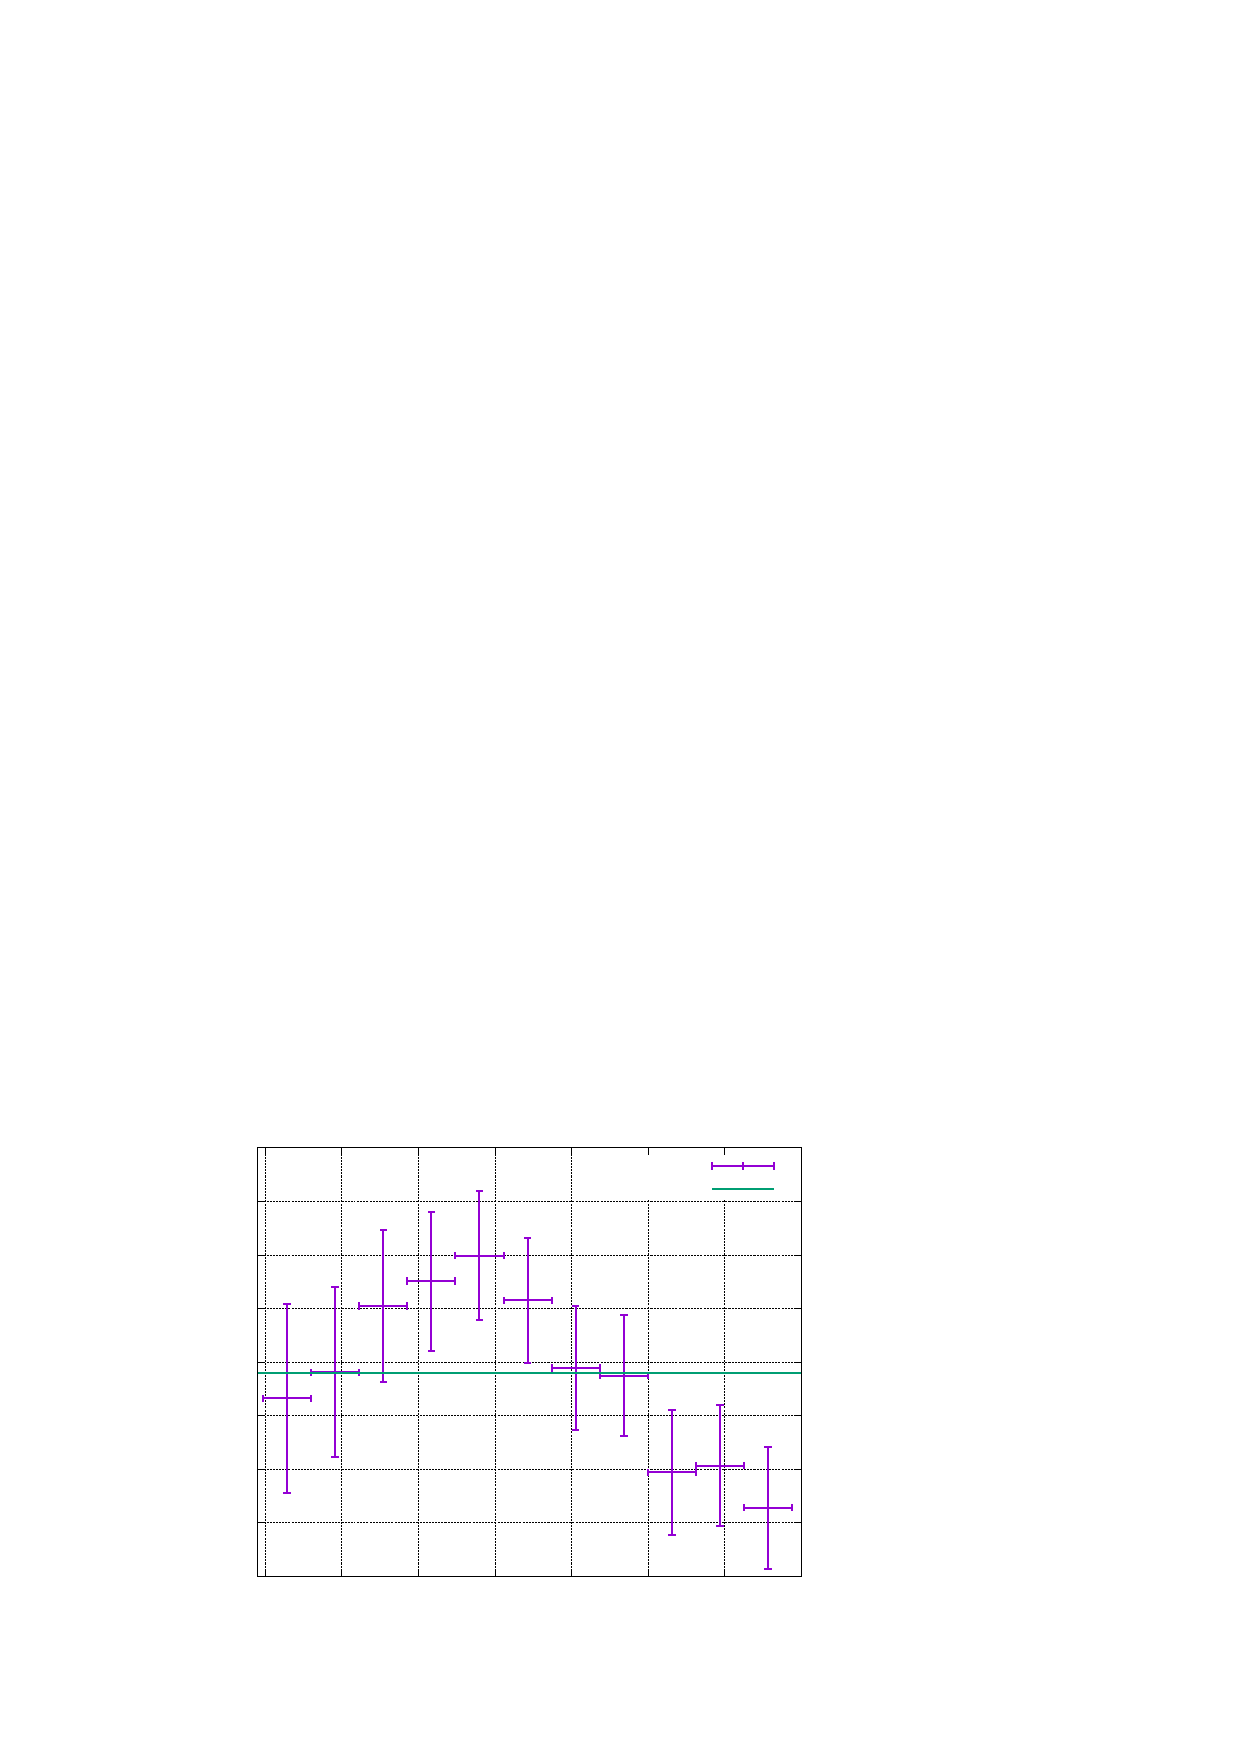
\includegraphics[width={360.00bp},height={252.00bp}]{nutation2}}%
    \gplfronttext
  \end{picture}%
\endgroup
}
    \caption{Nutation}
\end{figure}\\
Es ist zu erkennen, dass die gefittete Linie ($f(x)=ax+b$; $a=\left(-2,32\pm0,97\right)\cdot10^{-5}$;\\$b=\left(17,1\pm0,9\right)\cdot10^{-3}$) beinahe eine Parallele zur x-Achse ist.
Dies ist auch richtig, da das Verhältnis von $\omega_n$ zu $\omega_3$ druch die Träghietsmomente des Kreisels gegeben sind und sich diese während der Nutation nicht ändern können.\\
Nun wird der Mittelwert des Verhältnisses uns sein Fehler berechnet:
\begin{align*}
    \overline{\frac{\omega_\text{n}}{\omega_3}}&=\frac{1}{11}\cdot\sum_{\text{i}=1}^{11}\left(\frac{\omega_\text{n}}{\omega_3}\right)_\text{i}\\
    &=-0,017101093\\\\
    s_{\overline{\frac{\omega_\text{n}}{\omega_3}}}&=\sqrt{\sum_{\text{i}=1}^{11}\left(\frac{\partial\overline{\frac{\omega_\text{n}}{\omega_3}}}{\partial\left(\frac{\omega_\text{n}}{\omega_3}\right)_\text{i}}\cdot \left(s_{\frac{\omega_\text{n}}{\omega_3}}\right)_\text{i}\right)^2}\\
    &=\frac{1}{11}\sqrt{\sum_{\text{i}=1}^{11}\left(s_{\frac{\omega_\text{n}}{\omega_3}}\right)_\text{i}^2}\\
    &=0,0001960942
\end{align*}
Somit folgt:
\begin{equation*}
    \frac{J_3-J_1}{J_3}=-0,01710\pm0,00020
\end{equation*}